\chapter{Introduction}

\subsection{Our Contributions}

When Ono gave a survey on intermediate logics, which are logics between
intuitionistic and classical logics,
he \fix{cite} declared that he chose to study intermediate logics in
general rather than studying specific logics.
Since general results are logically stronger than concrete results,
theoretical scientists seek general results.
However, concrete results about specific subjects matter when the results
contain new phenomena.
This thesis is intended to contain such a concrete discovery.

Our subject is a typical intermediate logic called G\"odel--Dummett
logic, known since 1950's.
Our method is the Curry--Howard correspondence, also known since 1940's.


this is a replay of Curry's expression of surprise.

Of course, there have been many replays of Curry--Howard correspondence.


The Curry--Howard isomorphism~\citep{curryhoward} was first made
precise~\citep[p.97]{curryhoward} by \citet[\textbf{9}E and
\textbf{9}F]{curry1974combinatory}.
The intuitionistic propositional logic and the typed lambda calculus
had been independently invented but Curry discovered them to be the same thing.
The ``double discovery'' (\citet{wadler2012propositions}) is considered
to affirm the importance of the typed lambda calculi.
In this thesis we witness a replay of the ``double discovery'' with
different casts: G\"odel--Dummett logic and the waitfreedom.
Both of these were born in the early eras of their respective academic
disciplines:
mathematical logic bore G\"odel Dummett logic in
1950's~\citep{dummett59}
and the
computer science bore waitfree computation in
1970's~\citep{lamport1979make}.
This thesis is about the unknown connection between these two.

We list our contributions from the most important:
\begin{enumerate}
 \item identifying the computational ability of the
G\"odel--Dummett logic with waitfreedom (Chapter~\ref{ch:lambda}),
 \item developing a lambda calculus using
       a hypersequent calculus (Chapter~\ref{ch:lambda}),
 \item identifying the communication performed by the prelinearity axiom
       of monoidal t-norm logic (Chapter~\ref{ch:pole}),
 \item developing a parametricity argument for
       concurrent processes performing waitfree communication (Chapter~\ref{ch:pole}),
 % \item identifying the communication performed by a seemingly unknown axiom
 %       $(p\limp q)\otimes(q\limp p)$ on top of multiplicative linear
 %       logic (Chapter~\ref{ch:exchange}),
 \item finding a method for implementing hypersequent-based lambda calculi in a
       functional programming language Haskell on the Glasgow Haskell
       Compiler (Chapter~\ref{ch:haskell}).
\end{enumerate}

Our first contribution relies on our second contribution, which
develops a lambda calculus based on \citet{avron91}'s hypersequent
calculus for G\"odel--Dummett logic.  This justifies our title ``a
computational interpretation of G\"odel--Dummett logic.''
We found a way to interpret proofs in G\"odel--Dummett logic as
concurrently executable programs for waitfree computation.
Although \citet{avron91} noticed his hypersequent calculus has something
to do with concurrency (as the title of~\citep{avron91} contains the phrase
``intermediate logics for concurrency''), it was unknown that
the computational interpretation of G\"odel--Dummett logic has
the degree of synchronization called waitfreedom.  This discovery
constitutes our first contribution.
This is also important because it is the first such computational
interpretation for intermediate logics (Fig.~\ref{fig:lattice}).
 \begin{figure}
  \centering
  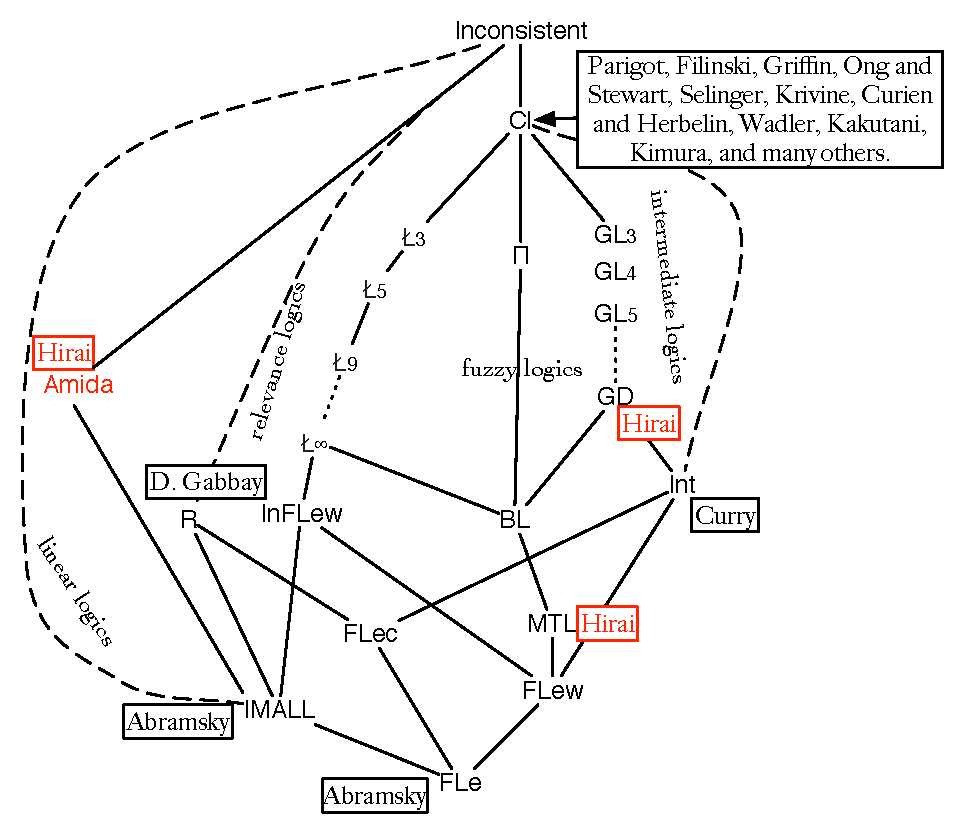
\includegraphics{lattice.eps}
  \caption[The substructural logics with lambda calculi.]
  {The substructural logics for which lambda calculi are found.
  The underlying Hasse diagram of well-known substructural logics is
  taken from
  \cite[p.~120]{residuated} with slight modifications.
  The names in boxes refer to people who developed lambda-calculi for
  these logics.
  \textsf{GD} stands for G\"odel--Dummett logic, for which
  a lambda calculus will be given in
  Chapter~\ref{ch:lambda}.
  \textsf{MTL} stands for monoidal t-norm logic~\citep{Esteva2001271},
  for which a lambda calculus will be given
  in Chapter~\ref{ch:pole}.
  \textsf{FLe} is for the full Lambek calculus with exchange
  rule~\citep[p.86]{residuated}, which is also known as the
  intuitionistic
  multiplicative additive fragment of linear logic (IMALL).
  \textsf{MALL} stands for its classical version, the multiplicative
  additive fragment of linear logic.  For these fragments of linear
  logic,
  \citet{abramsky1993computational} gave lambda calculi.
  \textsf{R} stands for relevance logic~\citep{urquhart1972},
  for which \citet{gabbay1992} gave a lambda calculus.
  \textsf{Int} stands for the intuitionistic propositional logic.
  The original Curry--Howard isomorphism was found for this logic by
  Curry~\citep{curry1942}.
  \textsf{Cl} stands for the classical propositional logic.
  There is intensive research going on for the computational
  interpretation of classical logic.  Namely,
  Parigot's $\lambda\mu$-calculus~\citep{lambdamu},
  Filinski's symmetric lambda calculus~\citep{filinski1989},
  Griffin's control perator~$\mathcal C$~\citep{griffin1990},
  Ong and Stewart's $\lambda\mu_{\mathrm
  v}$~\citep{ong-stewart},
%   \citet{bb1994}, this is predicate logic
  Selinger's categorical semantics and duality
  result~\citep{selinger2001} for which \citet{kakutani2002} introduced
  fixed-point
  operators,
  Curien and Herbelin's $\bar\lambda\mu\tilde\mu$
  calculus~\citep{curien2000},
  Wadler's dual calculus~\citep{wadler-dual, wadler-reloaded} and so on.
  For the history of lambda calculi for classical logic,
  Daisuke Kimura's thesis~\cite{kimura} is a source of detailed
  information.
  \textsf{Inconsistent} stands for the logic of all logical formulae.
  Notably, one programming language \texttt{Haskell}, which is based on
  the typed lambda calculi, has
  an inconsistent type system.
  }
  \label{fig:lattice}
 \end{figure}

The lambda calculus relies on \citet{avron91}'s hypersequents.
The hypersequent calculus is a
variant of the deduction system called sequent calculus.  In sequent
calculus, each step of a proof tree concludes a sequent $\G\vdash\phi$ that
consists of a finite sequence of logical formulae~$\G$ and a logical
formula~$\phi$.  After proving soundness of a sequent calculus, we know
that whenever a proof tree concludes $\G\vdash\phi$, any state of any model
satisfying all logical formulae in $\G$ must also satisfy the
formula~$\phi$.  In other words, the sequent $\G\vdash\phi$ is
interpreted as an implication.  In hypersequent calculus, each step of a
proof tree concludes a hypersequent instead of a sequent.  A
hypersequent is a sequence of sequents: $\G\vdash\phi\hmid \D\vdash\psi
\hmid \cdots$.  Also here, each component is interpreted as an
implication, and then the whole hypersequent is interpreted as the
disjunction of all those implications.
When we interpret proofs as programs, we take the components as
concurrent processeses.  Following the original disjunctive
interpretation of components, we regard the proof tree as the guarantee of
success of at least one process.

Our third contribution treats the prelinearity axiom
$(\phi\limp\psi)\oplus(\psi\limp\phi)$, which is the linear version of
Dummett's axiom.

Our fourth contribution is about the parametricity in the second-order
setting.  When we allow logical formulas to have quantifiers on
propositional variables (e.g. $\forall X(X\imp X)$), the logic gets much
more expressive.
Moreover, these second-order types can give more detailed specification
of programs than just specifying the types of outputs given types of
inputs.
For example, in \fix{specify logic}, a term of type $\forall X(X\imp X)$
must be the identity function.
Intuitively, since the term has to work on any type~$X$, the term cannot
look inside the argument of type~$X$.
Using this technique, we find the common behaviour of terms of type
$\forall X \forall Y ((X\limp Y)\lor (Y\limp X))$, thus finding the
computational semantics of Dummett's axiom.
Our technical development here is very similar to that of
\citet{danos-krivine}.  The crucial difference is that the processes do
not communicate in the case of \citet{danos-krivine} but they perform
waitfree communication in our case.


\fix{add nth and nth}

Our \fix{nth} contribution is a confirmation of our second contribution.
We implemented the lambda calculus on top of
Glasgow Haskell Compiler.

Our \fix{nth} contribution is about proof searching, which is another
kind of computation arising from propositional logic.
The lambda calculi is about removing detours from proofs while the proof
searching is about finding a proof or a counterexample for a given
conclusion.  \fix{read synch schemes paper and make regorous}
We are now able to connect our work with the tradition of
synchronization schemes.

\fix{where to put it}
Proofs as objects de Bruijin.

% \section{An Introduction for Computer Scientists}

% \section{An Introduction for Proof Theorists}

% \section{An Introduction for Functional Programmers}

% \section{An Introduction for Philosophers}

